\documentclass{article}
\usepackage[utf8]{inputenc}
\usepackage{graphicx}
\usepackage{here}

\title{TC5 : Traitement des images et du signal}

\author{Adrien Pavao}
\date{Septembre 2017}

\begin{document}

\maketitle

\tableofcontents

\section{Notions}

\begin{itemize}

\item Relation
\item Linéaire : Relation entre X et Y sous la forme Y = a X + b
\item Invariant par translation
\item Réponse impulsionnelle
\item 
L2 fonction -> continu
l2 suite -> discret
\item Signaux, energie, formule...
\item Occlusion
\item Quantification
\item Sténopé; chaine de traitements numérique pour s'en approcher en pratique
\item Théorème fondamental de la photographie, photons, photo-recepteurs, variables aléatoire de Poisson
\item Bruit (/!\ un peu de bruit -> efficacité sale possible)


\item \textbf{Convolution : } Le produit de convolution est un opérateur, généralement noté \textbf{*}, qui, à deux fonctions f et g sur un même domaine infini, fait correspondre une autre fonction \textbf{f * g} sur ce domaine, qui en tout point de celui-ci est égale à l'intégrale sur l'entièreté du domaine (ou la somme si celui-ci est discret) d'une des deux fonctions autour de ce point, pondérée par l'autre fonction autour de l'origine.

\begin{figure}[H]
   \caption{Schéma représentatif de la convolution d'une fonction porte par elle-même}
    \begin{center} 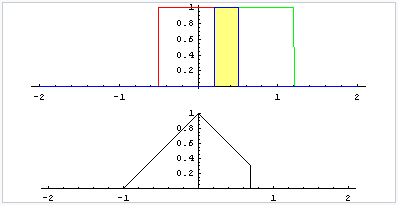
\includegraphics[scale=0.7]{convolution.png} \end{center}
\end{figure}

\begin{itemize}

\item Pour deux fonctions réelles ou complexes \textit{f} et \textit{g} :
\[ (f * g)(x) = game \]

\item Pour des suites : 
\[ (f * g)(n) = game \]

\end{itemize}


\item Universalité de la convolution

\item Transformée de Fourrier, série de fourrier, TFD
\item Hypothèse/Théorème Shannon / Shannon-Whittaker, fonctions 'bande limitée'
\item Normalisation

\item Filtre

\item \textbf{Théorème de Shannon (théorème d'échantillonage)}

On souhaite passer du continu au discret. Pour certaines fonctions, il est possible de pouvoir repasser du discret au continu (par exemple les fonctions à bornes limitées). 

\end{itemize}

\end{document}
